% The "%" character denotes a comment
\documentclass[prb,preprint]{revtex4-1}
\usepackage{amsmath}  % needed for \tfrac, \bmatrix, etc.
\usepackage{amsfonts} % needed for bold Greek, Fraktur, and blackboard bold
\usepackage{graphicx} % needed for figures
\usepackage{url}
\usepackage{float}

\newcommand{\dev}{LSM9DS1} % use "\dev" so you don't have to type LSM9DS1 every time

\begin{document}
\title{Microprocessors - Lab 05 Task 1}
\author{Adam Stammer}
%\email{adam.stammer@go.winona.edu}

\date{\today}

%if you include an abstract, it goes here
\begin{abstract}
This lab focuses on the basic use of the accelerometer on the LSM9DS1. My end goal was a tool that could be equipped into a package and shipped. If the box was mishandled, this type of sensor could be used to build that. First I aimed just to sense when the device was flat on the table. Next I was able output this data to an LCD. From there I added extra directional sensing (sideways, upsidedown, and anything else).
\end{abstract}

\maketitle
%title page ends here




\section{Up}
First, to wire it up was quite simple. I chose to use I2C, knowing that it only took 4 cables and because the SPI pins were not soldered onto the board. The I2C connections were properly labeled. SDA to SDA, SLC to SLC, GND to GND and VCC to 3.3V. I won't bother with a schematic because of how obvious that was. The datasheet helped determine the proper voltage at this point, but it was also necessary to figure out which axis to use to find which orientation was up. I've seen my share of confusing datasheets but this one is definitely up there. The orientation diagram seen below certainly helped, but as you can see the magnetometer is rotated 90 degrees from the other diagrams. That could clearly confuse somebody trying to use more than one of these sensors.

\begin{figure}[H]
	\centering
	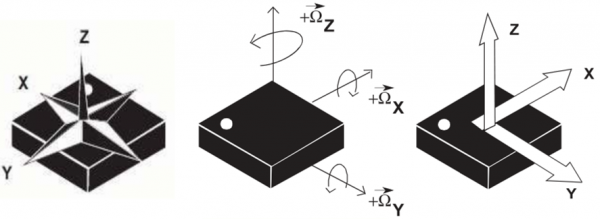
\includegraphics[width=5.75in]{axes.png}
	\caption{\dev Axis Orientation}
	\label{fig1}
\end{figure}

As you can see a positive Z indicates up, and the measurements are in Gs, so a Z measurement of +1, would indicate a straight up orientation with gravity pulling down against the sensor. Using the test example code from the \dev Arduino Library, I saw that this was indeed the case. In the process I noticed that the gyroscope was not working the way I expected it. More on this in the final section of this report.

I used the same LED hookup from the last lab to indicate up. I decided that any Z input that is 1 $\pm$ .05 would be considered up. This would turn on the led, and send an "UP!" signal through the Serial Monitor every quarter of a second. A video of this in action can be see at \url{https://mediaspace.minnstate.edu/media/Up+Detection+-+accl.+/1_5d5j3bcc}.

\section{LCD}
Combining the Liquid Crystal Display setup code form the previous lab, it was easy enough to print data to the LCD. Even though the Z axis was the only data relevant at the time, I knew the other axes would come in handy in the next phase of this lab. Adding a bit of code the existing if/else checking for up orientation, enabled an "UP!" or "NOT UP!" on the LCD as well. This made it even easier to see how the .05 buffer around the 1G was working. Any tighter of a window and I imagine the LED would've just been flickering, but too much bigger and I don't know if "UP" would've been the right descriptor. A video of this in action can be seen at \url{https://mediaspace.minnstate.edu/media/Up+Detection+-+accl.+With+LCD/1_q1khj3tr}.



\section{More Directions}
Next, I wanted a more practical application of this. Trying to think of something that needs to stay in an upright orientation I imagined a package that says "This Way Up $\uparrow$". I've seen mechanical devices (some of them using sand in specially shaped containers) that serve as indicators of how well a package like this was handled in shipping. ButI don't think just UP and NOT UP are good enough for this. It would be good to know how much time was spent in which orientation.

To accomplish this, I added more directions than just UP/NOT UP. Starting with the easiest, if Z was around -1 instead of +1, we know that it's upside down. This check was almost identical to the UP check. After that I checked for a SIDEWAYS orientation. A full $\pm$1G on either the X or Y axis would indicate this. To make the check simpler, I used the arduino's built in absolute value function (abs). This shrunk the logical checks on these axes by half. Moving the led logical status, and the LCD output message, outside of the scope of the if statements, simplified both considerably. You can see this in the main loop of the code associated with this report. A video demonstrating this can be found at \url{https://mediaspace.minnstate.edu/media/Orientation+Detector+-+Package+Handling+-+Accl+-+with+LCD/1_9lehslye}.

To finish up this kind of project, I would have to add some kind of data reporting. There are wireless transcievers that interface with the arduino, though I think only the SIM Card based devices would be applicable here. This would cost a good bit to use, especially since you likely wouldn't get the device back unless you're shipping something to yourself. Unless the package was very valuable, this wouldn't be worth it. It would be considerably cheaper to use an SD card reader/writer, but this would require retrieving the SD card, so again, unless the package was quite expensive, this wouldn't be worth it either. I imagine that's why this kind of a device isn't already being used. Nonetheless this was a fun project, and my first personal experience programming an accelerometer. 

An additional concern, is that measuring acceleration is not the best way to measure orientation. It works well when stationary and gravity is well defined by 1G, thus not requiring calibration or a starting orientation, but can cause plenty of problems when accelerating from some non gravity related means. I don't think that mail trucks tend to accelerate by the same acceleration as gravity, so maybe this wouldn't be a problem in most cases, but it's certainly not a baseless concern. Even driving up a hill could really mess it up, and probably report LIMBO. It would've been fun to use the gyroscope instead, maybe even in conjunction with the accelerometer to determine hills. I've never used a gyroscope before either, but running the test code, it keeps reporting crazy jumps. Without even moving it, or just moving it a tiny bit, and the report will jump sometimes a hundred degrees or more. Since my focus was on the accelerometer, I didn't care to debug it, but it's interesting to think about how I could've applied it to a project like this. Just being able to accomplish the same task with totally different sensors is pretty neat.



%\begin{thebibliography}{99}
% The numeral (here 99) in curly braces is nominally the number of entries in
% the bibliography. It's supposed to affect the amount of space around the
% numerical labels, so only the number of digits should matter--and even that
% seems to make no discernible difference.
%Not Requested
%\end{thebibliography}

\end{document}
